% Figure 1 — Matchstick Analogy: independence of the three terms
% TikZ port of docs/research/thinking/matchstick_figure_v2.html (Tier 1 task B)
% Standalone: compile with pdflatex for a cropped PDF, then \includegraphics,
% or paste the tikzpicture body into the paper with the color definitions.
% Color code (matches poster/HTML): EPC=coral (metric), dH=teal (measure),
% dB1=purple (topology).
\documentclass[tikz,border=8pt]{standalone}
\usepackage{amsmath}
\usetikzlibrary{positioning}

\definecolor{epcC}{RGB}{196,90,45}   % #c45a2d  EPC / metric
\definecolor{hC}{RGB}{42,107,138}    % #2a6b8a  dH / measure
\definecolor{bC}{RGB}{107,47,160}    % #6b2fa0  dB1 / topology
\definecolor{lossC}{RGB}{198,40,40}  % #c62828  loss / collapse

\begin{document}
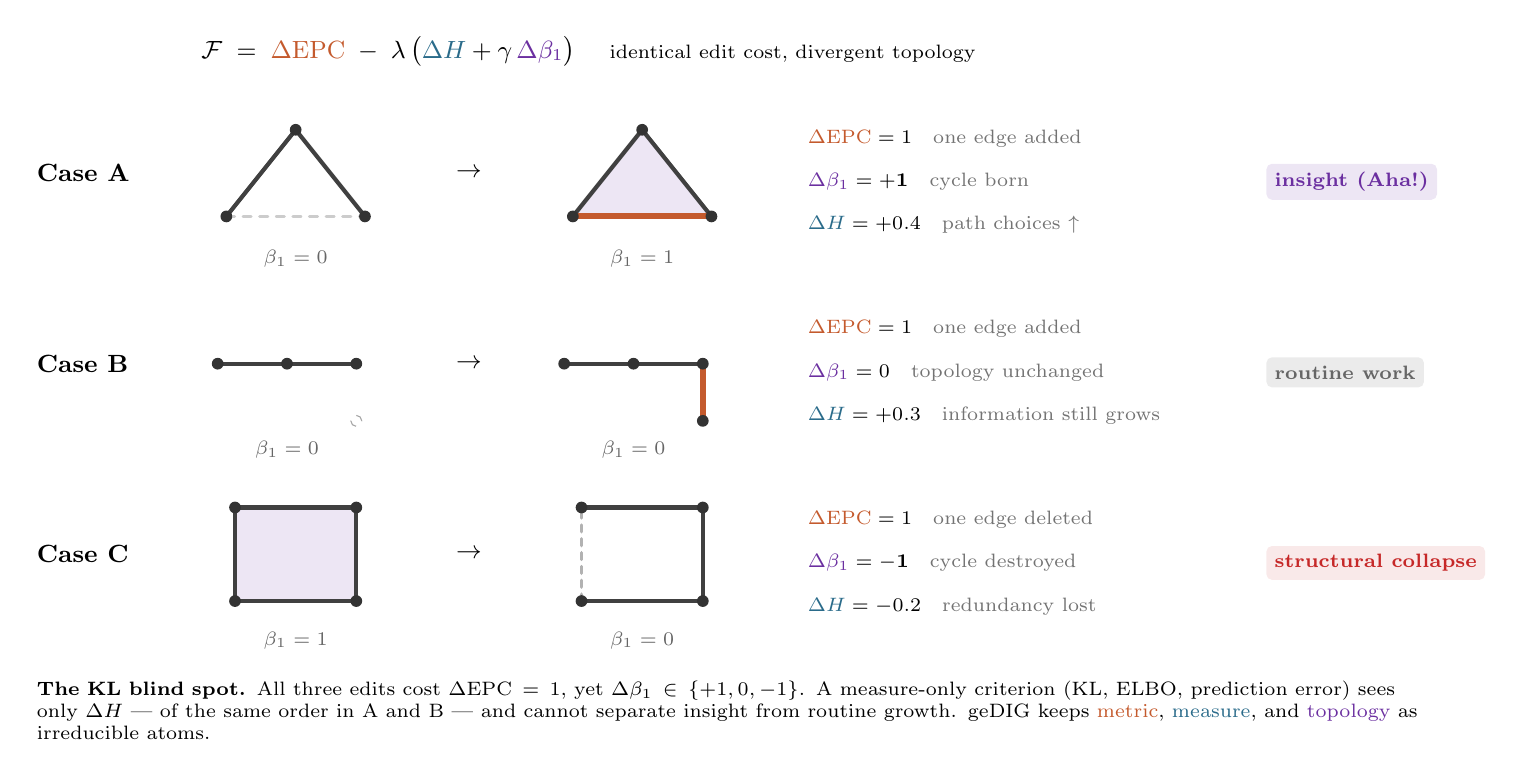
\begin{tikzpicture}[
  gnode/.style={circle, fill=black!80, inner sep=1.5pt},
  ghost/.style={circle, draw=black!35, dashed, inner sep=1.4pt},
  stick/.style={line width=1.5pt, draw=black!75, line cap=round},
  dimstick/.style={line width=1.0pt, draw=black!20, dashed, line cap=round},
  newedge/.style={line width=2.2pt, draw=epcC, line cap=round},
  removededge/.style={line width=1.2pt, draw=black!30, dash pattern=on 2.5pt off 2.5pt, line cap=round},
  caselabel/.style={font=\bfseries\small, anchor=west},
  blabel/.style={font=\scriptsize, text=black!60, anchor=north},
  metric/.style={font=\scriptsize, anchor=west},
  badge/.style={font=\scriptsize\bfseries, anchor=west, rounded corners=2pt, inner sep=3pt},
  x=0.022cm, y=0.022cm  % SVG pixel scale (viewBox 120x90); y pre-flipped below
]

% ---------- header formula ----------
\node[anchor=west, font=\small] at (0,335)
  {$\mathcal{F} \;=\; \textcolor{epcC}{\Delta\mathrm{EPC}} \;-\; \lambda\,\bigl(\textcolor{hC}{\Delta H} + \gamma\,\textcolor{bC}{\Delta\beta_1}\bigr)$
   \quad {\normalfont\scriptsize identical edit cost, divergent topology}};

% ============ Case A (row at y-offset 220): triangle completion ============
\node[caselabel] at (-95,265) {Case A};

\begin{scope}[shift={(0,220)}]  % before: open wedge, base edge only hinted
  \draw[stick] (20,20) -- (60,70);
  \draw[stick] (60,70) -- (100,20);
  \draw[dimstick] (20,20) -- (100,20);
  \node[gnode] at (20,20) {}; \node[gnode] at (60,70) {}; \node[gnode] at (100,20) {};
  \node[blabel] at (60,6) {$\beta_1 = 0$};
\end{scope}

\node[font=\small] at (160,265) {$\rightarrow$};

\begin{scope}[shift={(200,220)}]  % after: closing edge added, cycle born
  \fill[bC!12] (20,20) -- (60,70) -- (100,20) -- cycle;
  \draw[stick] (20,20) -- (60,70);
  \draw[stick] (60,70) -- (100,20);
  \draw[newedge] (20,20) -- (100,20);
  \node[gnode] at (20,20) {}; \node[gnode] at (60,70) {}; \node[gnode] at (100,20) {};
  \node[blabel] at (60,6) {$\beta_1 = 1$};
\end{scope}

\node[metric] at (350,285) {$\textcolor{epcC}{\Delta\mathrm{EPC}} = 1$ \; {\color{black!55}one edge added}};
\node[metric] at (350,260) {$\textcolor{bC}{\Delta\beta_1} = \mathbf{+1}$ \; {\color{black!55}cycle born}};
\node[metric] at (350,235) {$\textcolor{hC}{\Delta H} = +0.4$ \; {\color{black!55}path choices $\uparrow$}};
\node[badge, fill=bC!12, text=bC] at (620,260) {insight (Aha!)};

% ============ Case B (row at y-offset 110): path extension ============
\node[caselabel] at (-95,155) {Case B};

\begin{scope}[shift={(0,110)}]  % before: straight path, future node ghosted
  \draw[stick] (15,45) -- (55,45);
  \draw[stick] (55,45) -- (95,45);
  \node[gnode] at (15,45) {}; \node[gnode] at (55,45) {}; \node[gnode] at (95,45) {};
  \node[ghost] at (95,12) {};
  \node[blabel] at (55,6) {$\beta_1 = 0$};
\end{scope}

\node[font=\small] at (160,155) {$\rightarrow$};

\begin{scope}[shift={(200,110)}]  % after: one more edge, no cycle
  \draw[stick] (15,45) -- (55,45);
  \draw[stick] (55,45) -- (95,45);
  \draw[newedge] (95,45) -- (95,12);
  \node[gnode] at (15,45) {}; \node[gnode] at (55,45) {}; \node[gnode] at (95,45) {};
  \node[gnode] at (95,12) {};
  \node[blabel] at (55,6) {$\beta_1 = 0$};
\end{scope}

\node[metric] at (350,175) {$\textcolor{epcC}{\Delta\mathrm{EPC}} = 1$ \; {\color{black!55}one edge added}};
\node[metric] at (350,150) {$\textcolor{bC}{\Delta\beta_1} = 0$ \; {\color{black!55}topology unchanged}};
\node[metric] at (350,125) {$\textcolor{hC}{\Delta H} = +0.3$ \; {\color{black!55}information still grows}};
\node[badge, fill=black!8, text=black!60] at (620,150) {routine work};

% ============ Case C (row at y-offset 0): cycle edge deleted ============
\node[caselabel] at (-95,45) {Case C};

\begin{scope}[shift={(0,0)}]  % before: square with cycle
  \fill[bC!12] (25,72) -- (95,72) -- (95,18) -- (25,18) -- cycle;
  \draw[stick] (25,72) -- (95,72);
  \draw[stick] (95,72) -- (95,18);
  \draw[stick] (95,18) -- (25,18);
  \draw[stick] (25,18) -- (25,72);
  \node[gnode] at (25,72) {}; \node[gnode] at (95,72) {};
  \node[gnode] at (95,18) {}; \node[gnode] at (25,18) {};
  \node[blabel] at (60,6) {$\beta_1 = 1$};
\end{scope}

\node[font=\small] at (160,45) {$\rightarrow$};

\begin{scope}[shift={(200,0)}]  % after: left edge removed, cycle destroyed
  \draw[stick] (25,72) -- (95,72);
  \draw[stick] (95,72) -- (95,18);
  \draw[stick] (95,18) -- (25,18);
  \draw[removededge] (25,18) -- (25,72);
  \node[gnode] at (25,72) {}; \node[gnode] at (95,72) {};
  \node[gnode] at (95,18) {}; \node[gnode] at (25,18) {};
  \node[blabel] at (60,6) {$\beta_1 = 0$};
\end{scope}

\node[metric] at (350,65) {$\textcolor{epcC}{\Delta\mathrm{EPC}} = 1$ \; {\color{black!55}one edge deleted}};
\node[metric] at (350,40) {$\textcolor{bC}{\Delta\beta_1} = \mathbf{-1}$ \; {\color{black!55}cycle destroyed}};
\node[metric] at (350,15) {$\textcolor{hC}{\Delta H} = -0.2$ \; {\color{black!55}redundancy lost}};
\node[badge, fill=lossC!10, text=lossC] at (620,40) {structural collapse};

% ---------- footer: the KL blind spot ----------
\node[anchor=west, font=\scriptsize, text width=17.6cm, align=left] at (-95,-45)
  {\textbf{The KL blind spot.} All three edits cost $\Delta\mathrm{EPC}=1$, yet $\Delta\beta_1 \in \{+1, 0, -1\}$.
   A measure-only criterion (KL, ELBO, prediction error) sees only $\Delta H$ --- of the same order in A and B ---
   and cannot separate insight from routine growth. geDIG keeps
   \textcolor{epcC}{metric}, \textcolor{hC}{measure}, and \textcolor{bC}{topology} as irreducible atoms.};

\end{tikzpicture}
\end{document}
